\documentclass[12pt]{report}
\usepackage[utf8]{inputenc}
\usepackage[russian]{babel}
%\usepackage[14pt]{extsizes}
\usepackage{listings}
\usepackage{amsmath}
\usepackage[justification=centering]{caption}

\lstdefinelanguage{Kotlin}{
  comment=[l]{//},
  commentstyle={\color{gray}\ttfamily},
  emph={delegate, filter, first, firstOrNull, forEach, lazy, map, mapNotNull, println, return@},
  emphstyle={\color{OrangeRed}},
  identifierstyle=\color{black},
  keywords={abstract, actual, as, as?, break, by, class, companion, continue, data, do, dynamic, else, enum, expect, false, final, for, fun, get, if, import, in, interface, internal, is, null, object, override, package, private, public, return, set, super, suspend, this, throw, true, try, typealias, val, var, vararg, when, where, while},
  keywordstyle={\color{blue}\bfseries},
  morecomment=[s]{/*}{*/},
  morestring=[b]",
  morestring=[s]{"""*}{*"""},
  ndkeywords={@Deprecated, @JvmField, @JvmName, @JvmOverloads, @JvmStatic, @JvmSynthetic, Array, Byte, Double, Float, Int, Integer, Iterable, Long, Runnable, Short, String},
  ndkeywordstyle={\color{orange}\bfseries},
  sensitive=true,
  stringstyle={\color{green}\ttfamily},
}

% Для листинга кода:
\lstset{ %
language=Kotlin,                 % выбор языка для подсветки (здесь это С)
basicstyle=\footnotesize\sffamily, % размер и начертание шрифта для подсветки кода
numbers=left,               % где поставить нумерацию строк (слева\справа)
numberstyle=\tiny,           % размер шрифта для номеров строк
stepnumber=1,                   % размер шага между двумя номерами строк
numbersep=5pt,                % как далеко отстоят номера строк от подсвечиваемого кода
showspaces=false,            % показывать или нет пробелы специальными отступами
showstringspaces=false,      % показывать или нет пробелы в строках
showtabs=false,             % показывать или нет табуляцию в строках
frame=single,              % рисовать рамку вокруг кода
tabsize=2,                 % размер табуляции по умолчанию равен 2 пробелам
captionpos=t,              % позиция заголовка вверху [t] или внизу [b] 
breaklines=true,           % автоматически переносить строки (да\нет)
breakatwhitespace=false, % переносить строки только если есть пробел
escapeinside={\#*}{*)}   % если нужно добавить комментарии в коде
}

\usepackage{hyperref}
\hypersetup{
    linktoc=all,     %set to all if you want both sections and subsections linked
    linkcolor=blue,  %choose some color if you want links to stand out
}

% Для измененных титулов глав:
\usepackage{titlesec, blindtext, color} % подключаем нужные пакеты
\definecolor{gray75}{gray}{0.75} % определяем цвет
\newcommand{\hsp}{\hspace{20pt}} % длина линии в 20pt
% titleformat определяет стиль
\titleformat{\chapter}[hang]{\Huge\bfseries}{\thechapter\hsp\textcolor{gray75}{|}\hsp}{0pt}{\Huge\bfseries}

% plot
\usepackage{pgfplots}
\usepackage{filecontents}
\usetikzlibrary{datavisualization}
\usetikzlibrary{datavisualization.formats.functions}
\begin{filecontents}{KA0.dat}
100 2148121
200 17350292
300 68920554
400 211301483
500 367822853
600 678478122
\end{filecontents}

\begin{filecontents}{KV0.dat}
100 2302331
200 22592034
300 73453362
400 205981760
500 351730341
600 658012453
\end{filecontents}

\begin{filecontents}{UKV0.dat}
100 1921005
200 1425033
300 57000923
400 172968826
500 340284336
600 625149992
\end{filecontents}

\begin{filecontents}{KA1.dat}
101 2312114
201 20247410
301 75166547
401 227614782
501 364368768
601 672846913
\end{filecontents}

\begin{filecontents}{KV1.dat}
101 2623891
201 21694235
301 77955778
401 218087162
501 362588416
601 671159157
\end{filecontents}

\begin{filecontents}{UKV1.dat}
101 2032155
201 17554153
301 64421195
401 171881527
501 358108198
601 647843183
\end{filecontents}


\begin{document}
\begin{titlepage}
	\fontsize{12pt}{12pt}\selectfont
	\noindent \begin{minipage}{0.15\textwidth}
		
\includegraphics[width=\linewidth]{inc/img/b_logo.jpg}
	\end{minipage}
	\noindent\begin{minipage}{0.9\textwidth}\centering
		\textbf{Министерство науки и высшего образования Российской Федерации}\\
		\textbf{Федеральное государственное бюджетное образовательное учреждение высшего образования}\\
		\textbf{«Московский государственный технический университет имени Н.Э.~Баумана}\\
		\textbf{(национальный исследовательский университет)»}\\
		\textbf{(МГТУ им. Н.Э.~Баумана)}
	\end{minipage}
	
	\noindent\rule{15cm}{3pt}
	\newline\newline
	\noindent ФАКУЛЬТЕТ \underline{~~~~~~~~~~~~~~~~«Информатика и системы управления»~~~~~~~~~~~~~~~~} \newline\newline
	\noindent КАФЕДРА \underline{«Программное обеспечение ЭВМ и информационные технологии»}\newline\newline\newline\newline\newline\newline\newline
	
	
	\begin{center}
		\Large\textbf{Отчет по лабораторной работе №3 по курсу "Анализ алгоритмов"}\newline
	\end{center}
	
	\noindent\textbf{Тема} \underline{Алгоритмы сортировки}\newline\newline\newline
	\noindent\textbf{Студент} \underline{Якуба Д. В.}\newline\newline
	\noindent\textbf{Группа} \underline{ИУ7-53Б}\newline\newline
	\noindent\textbf{Оценка (баллы)} \underline{~~~~~~~~~~~~~~~~~~~}\newline\newline
	\noindent\textbf{Преподаватели} \underline{Волкова Л.Л., Строганов Ю.В.}\newline
	
	\begin{center}
		\vfill
		Москва~---~\the\year
		~г.
	\end{center}
\end{titlepage}

\tableofcontents

\newpage
\chapter*{Введение}
\addcontentsline{toc}{chapter}{Введение}
\section*{Цели лабораторной работы}
\begin{enumerate}
\item изучение алгоритмов сортировки пузырьком, вставками и выбором;
\item реализация алгоритмов сортировки пузырьком, вставками и выбором;
\item проведение сравнительного анализа трудоёмкости алгоритмов на основе теоретических расчетов и выбранной модели вычислений;
\item сравнительный анализ алгоритмов на основе экспериментальных данных;
\item подготовка отчёта по лабораторной работе;
\item получение практических навыков реализации алгоритмов на ЯП Kotlin.
\end{enumerate}
\section*{Определение}
Сортировка - это процесс перегруппироваки заданной последовательности объектов в некотором определённом порядке. Такой определённый порядок позволяет, в некоторых случаях, эффективнее работать с заданной последовательностью.

Пусть требуется упорядочить $N$ элементов: $E_1,E_2,...,E_n$. Каждый элемент представляет из себя запись $E_j$, содержащую некоторую информацию и ключ $K_j$, управляющий процессом сортировки. На множестве ключей определено отношение порядка $<$ так, чтобы для любых трёх значений ключей $a,b,c$ выполнялись следующие условия:

\begin{itemize}
\item Либо $a < b$, либо $b < c$, либо $a = b$;
\item Если $a < b$ и $b < c$, то $a < c$.
\end{itemize}

Данные условия определяют математическое понятие линейного и совершенного упорядочения, а удовлетворяющие им множества поддаются сортировке болшинством методов.

Задачей сортировки является нахождение такой перестановки записей $p(1)p(2)...p(n)$ с индексами ${1, 2, ..., N}$, после которой ключи расположились бы в порядке неубывания.

\begin{equation}
K_{p(1)} \leq K_{p(2)} \leq ... \leq K_{p(n)}
\end{equation}

\chapter{Аналитическая часть}

\section{Алгоритм сортировки пузырьком}
Алгоритм заключается в повторяющих проходах по сортируемому массиву. За каждый проход элементы последовательно сравниваются попарно. В том случае, если два элемента расположены не по порядку, то они меняются местами \cite{Knut}. Этот процесс повторяется до тех пор, пока элементы не будут упорядочены, то есть, в случае массива элементов размером $n$, проходы повторятся $n - 1$ раз.

\section{Алгоритм сортировки вставками}
Алгоритм заключается в следующей последовательности действий: элементы просматриваются по одному, и каждый новый элемент вставляется в подходящее место среди ранее упорядоченных элементов \cite{Knut}.

В начальный момент времени отсортированная последовательность пуста. На каждом шаге алгоритма выбирается один из элементов входных данных и помещается на нужную позицию в уже осотированной последовательности до тех пор, пока набор входных данных не будет исчерпан. В любой момент времени в отсортированной последовательности элеметы удовлетворяют требованиям к выходным данным алгоритма.

\section{Алгоритм сортировки выбором}
Алгорим заключается в следующей последовательности действий: сначала выделяется наименьший (наибольший) элемент последовательности и каким-либо образом отделяется от остальных, затем выбирается наименьший (наибольший) из оставшихся и т.д. \cite{Knut}

\section*{Вывод}
Были рассмотрены алгоритмы сортировки пузырьком, вставками и выбором. В данной работе стоит задача реализации рассмотренных алгоритмов. Также будет необходимо оценить теоретическую оценку алгоритмов и проверить её экспериментально.

\chapter{Конструкторская часть}
\section{Блок-схема алгоритма сортировки пузырьком}
Блок-схема алгоритма сортировки пузырьком предоставлена на рисунке \ref{img:bubbleSortScheme}.

\begin{figure}
\begin{center}
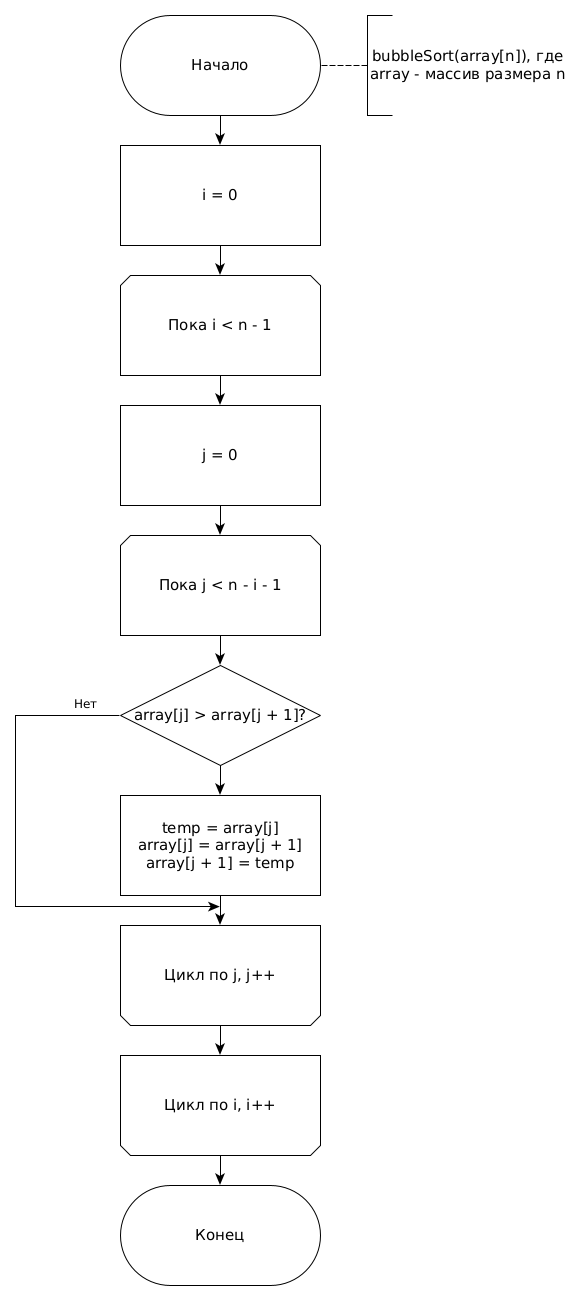
\includegraphics[scale=0.4]{inc/img/bubbleSort.png}
\captionsetup{justification=centering}
	\caption{Блок-схема алгоритма сортировки пузырьком.}
	\label{img:bubbleSortScheme}	
\end{center}
\end{figure}

\section{Блок-схема алгоритма сортировки вставками}
Блок-схема алгоритма сортировки вставками предоставлена на рисунке \ref{img:insertionSortScheme}.

\begin{figure}
\begin{center}
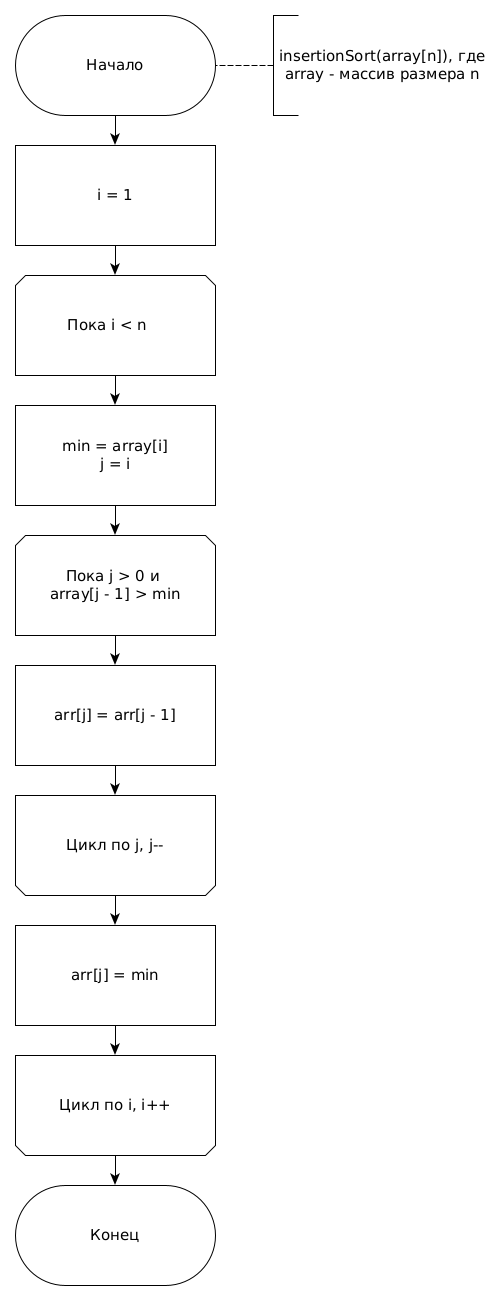
\includegraphics[scale=0.4]{inc/img/insertionSort.png}
\captionsetup{justification=centering}
	\caption{Блок-схема алгоритма сортировки вставками.}
	\label{img:insertionSortScheme}	
\end{center}
\end{figure}

\section{Блок-схема алгоритма сортировки выбором}
Блок-схема алгоритма сортировки выбором предоставлена на рисунке \ref{img:selectionSortScheme}.

\begin{figure}
\begin{center}
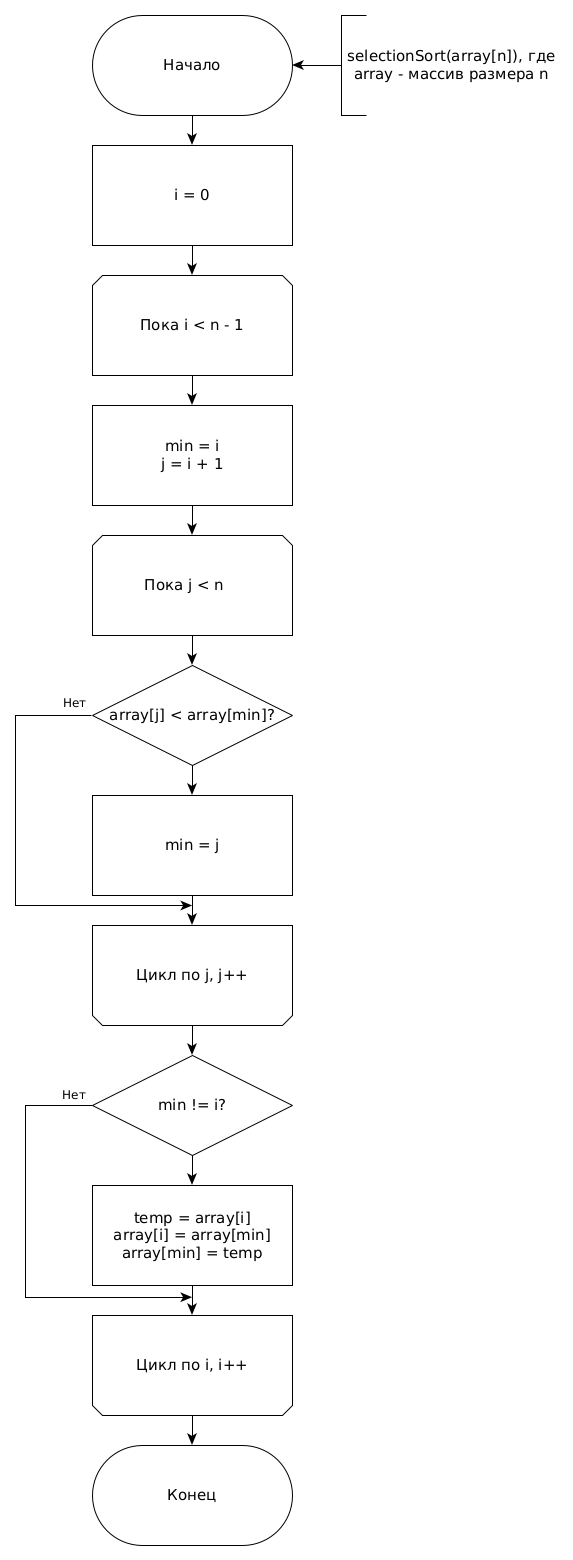
\includegraphics[scale=0.33]{inc/img/selectionSort.png}
\captionsetup{justification=centering}
	\caption{Блок-схема алгоритма сортировки выбором.}
	\label{img:selectionSortScheme}	
\end{center}
\end{figure}

\newpage

\section{Модель вычислений}

\section{Трудоёмкость алгоритмов}
\subsection{Алгоритм сортировки пузырьком}

\subsection{Алгоритм сортировки вставками}

\subsection{Алгоритм сортировки выбором}

\section*{Вывод}
На основе теоретичесих данных, полученных из аналитического раздела, были построены схемы рассматриваемых алгоритмов сортировок, оценены их трудоёмкости в лучшем и худшем случаях.

\chapter{Технологическая часть}
\section{Требования к программному обеспечению}
Программное обеспечение принимает на вход массив целочисленных значений.

В результате выполнения программы должен быть получен упорядоченный по возрастанию массив.

\section{Средства реализации программного обеспечения}
При написании программного продукта был использован язык программирования Kotlin \cite{Kotlin}.

Данный выбор обусловлен следующими факторами:
\begin{itemize}
\item Высокая вычислительная производительность;
\item Большое количество справочной литературы, связанной с ЯП Java.
\end{itemize}

Для тестирования производительности реализаций алгоритмов использовалась утилита measureTimedValue.

При написаннии программного продукта использовалась среда разработки IntelliJ IDEA.

Данный выбор обусловлен тем, что язык программирования Kotlin - это разработка компании JetBrains, поставляющей данную среду разработки.

\section{Листинг кода}
В листингах \ref{list:bubbleSort} - \ref{list:selectionSort} предоставлены реализации рассматриваемых алгоритмов.
\begin{lstlisting}[caption=Функция реализации алгоритма сортировки пузырьком,
label={list:bubbleSort}]
fun bubbleSort(arr: IntArray)
{
    var i = 0;
    while (i < arr.size - 1)
    {
        var j = 0;
        while (j < arr.size - 1 - i)
        {
            if (arr[j] > arr[j + 1])
                arr[j + 1] = arr[j].also { arr[j] = arr[j + 1] }
            j++
        }
        i++
    }
}
\end{lstlisting}

\begin{lstlisting}[caption=Функция реализации алгоритма сортировки вставками,
label={list:insertionSort}]
fun insertionSort(arr: IntArray)
{
    var i = 2;
    while (i < arr.size)
    {
        var min = arr[i]
        var j = i;
        while (j > 0 && arr[j - 1] > min)
        {
            arr[j] = arr[j - 1]
            j--
        }
        arr[j] = min
        i++
    }
}
\end{lstlisting}

\begin{lstlisting}[caption=Функция реализации алгоритма сортировки выбором,
label={list:selectionSort}]
fun selectionSort(arr: IntArray)
{
    var i = 0;
    while (i < arr.size - 1)
    {
        var j = i + 1
        var min = i
        while (j < arr.size)
        {
            if (arr[j] < arr[min])
                min = j
            j++
        }
        if (min != i)
            arr[i] = arr[min].also { arr[min] = arr[i] }
        i++
    }
}
\end{lstlisting}

\section{Тестирование программного продукта}
В таблице~\ref{tests} приведены тесты для функций, реализующих алгоритм сортировки пузырьком, вставками и выбором. Тесты пройдены успешно.

\begin{table}[h!]
	\begin{center}
		\begin{tabular}{|c|c|c|}
			\hline
			Начальный массив & Ожидаемый результат & Полученный результат \\ 
			\hline
			$[5, 4, 3, 2, 1]$ & $[1, 2, 3, 4, 5]$  & $[1, 2, 3, 4, 5]$\\
			$[0, 0, 0]$  & $[0, 0, 0]$  & $[0, 0, 0]$\\
			$[1, 2, 3]$ & $1, 2, 3$ & $1, 2, 3$\\
			$[]$  & $[]$  & $[]$\\
			\hline
		\end{tabular}
		\caption{\label{tests}Тестирование функций}
	\end{center}
\end{table}
\section*{Вывод}
Спроектированные алгоритмы вычисления произведения двух матриц были реализованы и протестированы.

\chapter{Исследовательская часть}

\section{Пример работы программного обеспечения}
Ниже на рисунках \ref{img:exampleRand}- \ref{img:exampleInp} предоставлены примеры работы каждого из алгоритмов на случайных данных, сгенерированных один раз, и введённых пользователем данных.

\begin{figure}
\begin{center}
\captionsetup{justification=centering}
	\caption{Пример работы ПО.}
	\label{img:exampleRand}	
\end{center}
\end{figure}

\begin{figure}
\begin{center}
\captionsetup{justification=centering}
	\caption{Пример работы ПО.}
	\label{img:exampleInp}	
\end{center}
\end{figure}

\newpage

\section{Технические характеристики}
Технические характеристики ЭВМ, на котором выполнялись исследования:
\begin{itemize}
\item ОС: Manjaro Linux 20.1.1 Mikah
\item Оперативная память: 16 Гб
\item Процессор: Intel Core i7-10510U

При проведении замеров времени ноутбук был подключен к сети электропитания.
\end{itemize}

\section{Время выполнения алгоритмов}
Алгоритмы тестировались на данных, сгенерированных случайным образом один раз.

Результаты замеров времени приведены в таблице \ref{time}. На рисунках \ref{timeRes1} и \ref{timeRes2} приведены графики зависимостей времени работы алгоритмов от количества строк и столбцов матриц (в чётном и нечётном вариантах). В таблице СА - Сортировка Пузырьком, СВст - Алгоритм Копперсмита-Винограда, УКВ - Улучшенный Алгоритм Копперсмита-Винограда.

\newpage
\begin{table}[h]
	\begin{center}
		\caption{\label{time} Замеры времени для квадратных матриц различных размеров}
		\begin{tabular}{|c c c c|} 
 			\hline
			Размер матрицы & КА & КВ & УКВ \\ [0.5ex] 
 			\hline\hline
 			100 & 2148121& 2302331& 1921005\\
 			\hline
 			101 & 2312114& 2623891& 2032155\\
 			\hline
			200 & 17350292& 22592034& 1425033\\
			\hline
			201 & 20247410& 21694235& 17554153\\
			\hline
			300 & 68920554&  73453362& 57000923\\
			\hline
			301 &  75166547&  77955778& 64421195\\
			\hline
			400 &  211301483&  205981760& 172968826\\
			\hline
			401 &  227614782&  218087162& 171881527\\
			\hline
			500 &  367822853&  351730341& 340284336\\
			\hline
			501 &  364368768&  362588416& 358108198\\
			\hline
			600 &  678478122&  	658012453& 625149992\\
			\hline
			601 &  672846913&  671159157& 647843183\\
			\hline
			\end{tabular}
	\end{center}
\end{table}

\begin{figure}[h]
\begin{center}
	\begin{tikzpicture}

\begin{axis}[
  		  	axis lines = left,
  		  	xlabel = размер,
  		  	ylabel = {время, нс},
			legend pos=north west,
			ymajorgrids=true
		] 
		\addplot[color=orange] table[x index=0, y index=1] {KA0.dat};
		\addplot[color=blue, mark=square] table[x index=0, y index=1] {KV0.dat};
		\addplot[color=green, mark=square] table[x index=0, y index=1] {UKV0.dat};

		\addlegendentry{КА}
		\addlegendentry{КВ}
		\addlegendentry{УКВ}
		\end{axis}
	\end{tikzpicture}
	\captionsetup{justification=centering}
	\caption{Зависимость времени работы от размера матриц (чётные значения размерностей)}
	\label{timeRes1}
	\end{center}
\end{figure}

\begin{figure}[h]
	\begin{center}
	\begin{tikzpicture}

		\begin{axis}[
 		   	axis lines = left,
 		   	xlabel = размер,
 		   	ylabel = {время, нс},
			legend pos=north west,
			ymajorgrids=true
		]
		\addplot[color=orange] table[x index=0, y index=1] {KA1.dat};
		\addplot[color=blue, mark=square] table[x index=0, y index=1] {KV1.dat};
		\addplot[color=green, mark=square] table[x index=0, y index=1] {UKV1.dat};

		\addlegendentry{КА}
		\addlegendentry{КВ}
		\addlegendentry{УКВ}
		\end{axis}
\end{tikzpicture}
	\captionsetup{justification=centering}
	\caption{Зависимость времени работы от размера матриц (нечётные значения размерностей)}
	\label{timeRes2}
	\end{center}
\end{figure}

\section*{Вывод}
При сравнении результатов замеров времени заметно, что скорость работы классического алгоритма однозначно отстаёт от скорости работы улучшенного Алгоритма Копперсмита-Винограда. Уже на 600 элементах улучшенный алгоритм Копперсмита-Винограда работает быстрее классического на $\approx8\%$. При нечётном количестве строк и столбцов матриц улучшенный алгоритм способен быть медленнее $\approx4\%$, при факте того, что классический алгоритм похожей динамики не имеет. Обычный алгоритм Копперсмита-Винограда начинает выигрывать по скорости классический только по достижению 300 строк и столбцов в матрице, при факте того, что в случае матрицы с нечётной размерностью он всё ещё будет проигрывать. При размерности 600 он будет выгрывать у классической реализации на $\approx3\%$. В случае матриц размера меньше 400 на 400 его использование не будет целесообразным.

\chapter*{Заключение}
\addcontentsline{toc}{chapter}{Заключение}
В ходе выполнения лабораторной работы:
\begin{itemize}
\item были изучены алгоритмы умножения матриц: классический, Копперсмита-Винограда и улучшенный Копперсмита-Винограда;
\item были реализованы алгоритмы умножения матриц: классический, Копперсмита-Винограда и улучшенный Копперсмита-Винограда;
\item был произведён анализ трудоёмкости указанных алгоритмов на основе теоретических расчётов и выбранной модели вычислений;
\item был выполнен сравнительный анализ производительности алгоритмов на основе полученных экспериментальных данных;
\item был подготовлен отчёт по проделанной работе;
\item были получены практические навыки реализации алгоритмов на ЯП Kotlin.
\end{itemize}

Исследования показали, что использование алгоритма Копперсмита-Винограда способно оправдать себя только в случае матриц, размерность которых не менее 400. При этом выигрыш будет составлять $\approx0.2\%$ только в случае чётной размерности. Реализация улучшенного алгоритма Копперсмита-Винограда показывает результаты быстрее классического алгоритма уже при размерности матрицы 100. Чем больше элементов в матрице, тем заметнее разница во времени работы этих двух алгоритмов. При размерности матрицы 600 модифицированный алгоритм Копперсмита-Винограда показывает себя лучше классического алгоритма на $\approx8\%$.

\addcontentsline{toc}{chapter}{Литература}
\bibliographystyle{utf8gost705u}  % стилевой файл для оформления по ГОСТу
\bibliography{biblio.bib}          % имя библиографической базы (bib-файла)


\end{document} 
